\Chapter{A front end megvalósítása}

% TODO: Minden képet be kell majd hivatkozni!

% TODO: A szövegben ki kell emelni a kódrészeket texttt{}-vel! ..vagy textit-vel, csak következetes legyen!

\Section{Felhasználói felület elemei}

Az alkalmazás főoldalán egy ismertető található, a program funkcionalitását bemutatva.
A felhasználói felületének két fő része van, a menetrendadatok böngészése és az útvonaltervezés. Ezeket a navigációs sávon külön menüpontokból érhetjük el.

\begin{figure}[h!]
\centering
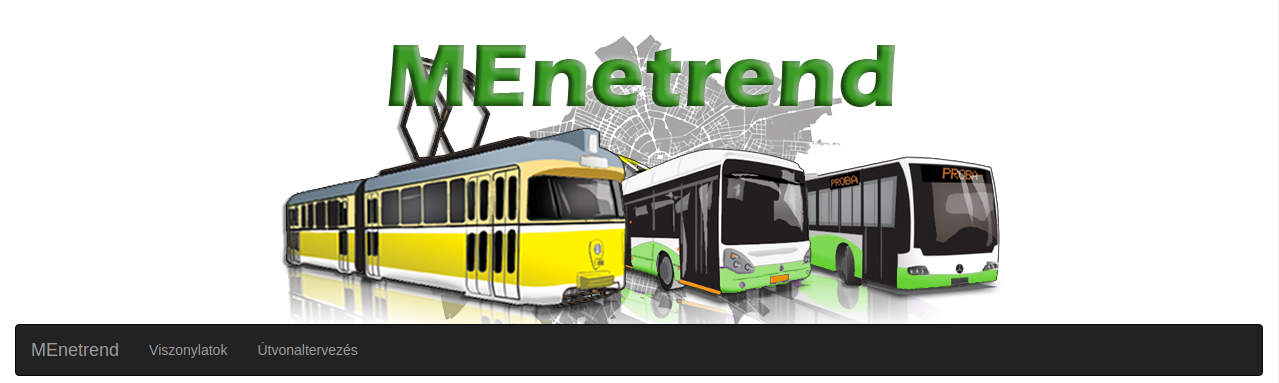
\includegraphics[scale=0.32]{kepek/navbar.png}
\caption{Az alkalmazás navigációs sávja}
\label{fig:navbar}
\end{figure}

A navigációs sávon (\ref{fig:navbar}. ábra) a Viszonylatok menüpontra kattintva láthatjuk a különböző viszonylatokat, ahol többféle módon is kiválaszthatjuk azt, amelyiknek a menetrendjére kíváncsiak vagyunk. Található az oldal tetején egy gombsor a vonalszámokkal (\ref{fig:viszonylatok_gombsor}. ábra), alatta pedig egy részletes táblázat, csoportosítva a különböző típusú viszonylatokat.

\begin{figure}[h!]
\centering
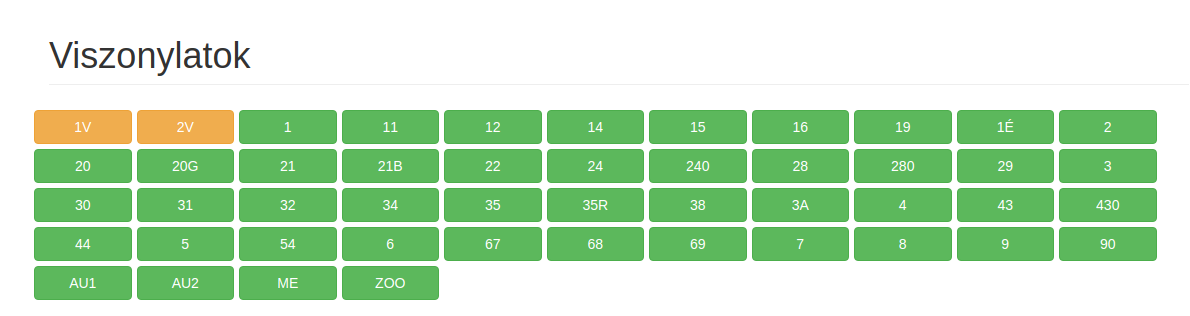
\includegraphics[scale=0.32]{kepek/viszonylatok_gombsor.png}
\caption{Gombsor a vonalszámokkal}
\label{fig:viszonylatok_gombsor}
\end{figure}

\Aref{fig:vonalak_tablazat}. ábrán látható táblázat három oszlopból áll: vonalszám, induló állomás és érkező állomás. Lehetőség van bármelyik oszlop szerint csökkenő vagy növekvő sorrendben rendezni a táblázatot vagy keresni benne. A Keresés mezőbe beírt szöveg alapján a táblázat mindegyik oszlopában keres egyezőséget, a szűrés az oldal újratöltése nélkül megtörténik. A keresés kis- és nagybetű-érzéketlen.

\begin{figure}[h!]
\centering
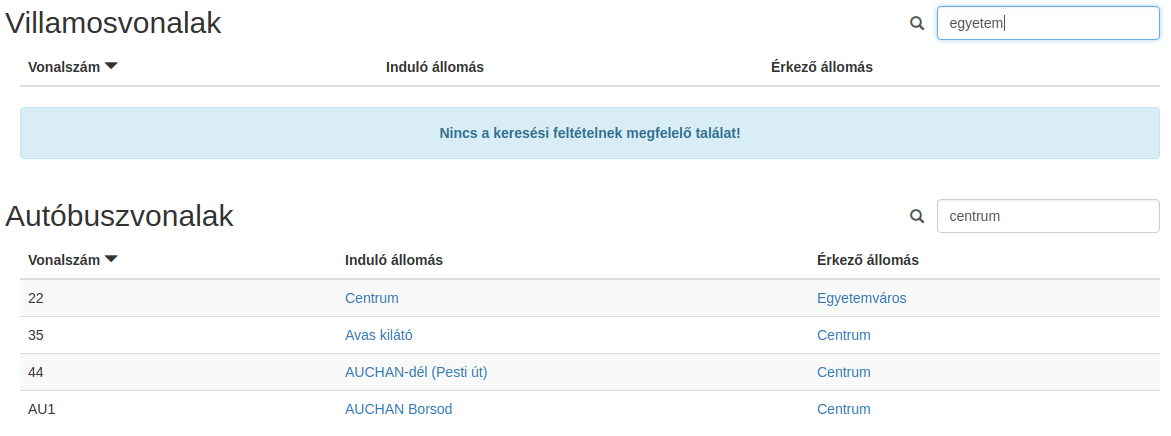
\includegraphics[scale=0.32]{kepek/vonalak_tablazat.png}
\caption{A vonalszámokat, indulóállomásokat és az érkező állomásokat megjelenítő táblázat}
\label{fig:vonalak_tablazat}
\end{figure}

Ha kiválasztunk egy viszonylatot, akkor annak az aznapi menetrendjét látjuk egy óra-perc táblázatban (\ref{fig:menetrend}. ábra). A táblázat mellett egy legördülő menüből lehet a napot választani, ha a vonal egy másik napi menetrendjére vagyunk kíváncsiak.

\begin{figure}[h!]
\centering
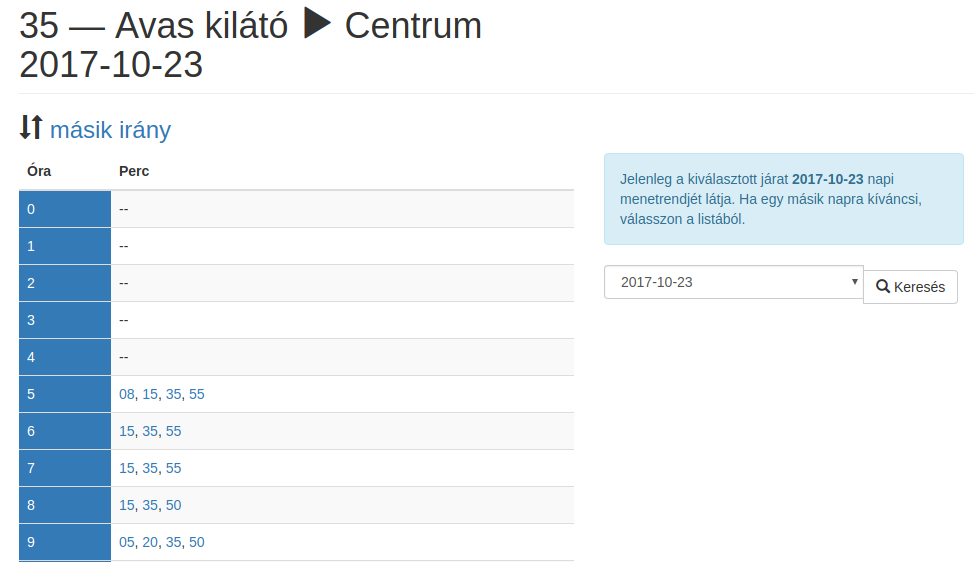
\includegraphics[scale=0.4]{kepek/menetrend.png}
\caption{Az adott nap menetrendje óra-perc táblázatos formában}
\label{fig:menetrend}
\end{figure}

A táblázatban a percek linkek, amire ha rákattintunk, akkor egy másik oldal töltődik be, amit \aref{fig:trip_tablazat_es_terkep}. ábrán láthatunk. Ez az oldal is két részre van felosztva. Bal oldalt egy táblázatban láthatjuk a kiválasztott járat részletes menetrendjét, sorrendben az állomásokat, amiket érint. Három oszlopból áll a táblázat: indulási idő, megálló neve, és az addigi menetidő percben kifejezve. A táblázat mellett pedig a járat útvonala jelenik meg Google Mapsen. A térképen a járat útvonala és az érintett megállók is fel vannak tüntetve. A megállókat jelző \texttt{markerekre} kattintva egy \texttt{InfoWindow} ugrik fel, a megálló nevét és a járat végállomását tartalmazva.

\begin{figure}[h!]
\centering
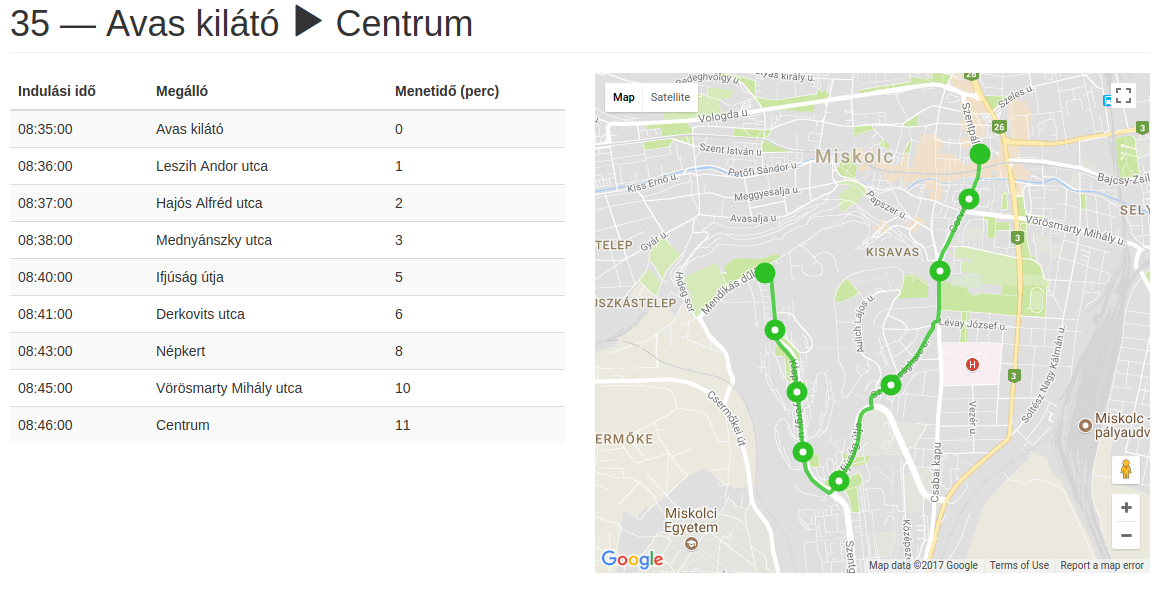
\includegraphics[scale=0.35]{kepek/trip_tablazat_es_terkep.png}
\caption{Egy járat megállóinak és útvonalának megjelenítése táblázatos és térképes formában}
\label{fig:trip_tablazat_es_terkep}
\end{figure}

Az alkalmazás másik fő funkcióját is a navigációs sávról érhetjük el, ez nem más, mint az útvonaltervezés. Az oldal két részre van felosztva, ahogy \aref{fig:trip_planner}. ábrán látható.

Bal oldalt az útvonaltervezés beállításait adhatjuk meg. Az első sorban a kezdő- és a célmegállót állíthatjuk be két beviteli mező segítségével, amit \textit{autocomplete} támogatás is segít. Ez azt jelenti, hogy ha elkezdünk gépelni a beviteli mezőbe, akkor megjelenik egy legördülő listához hasonlító elem, amiből kiválaszthatjuk a megfelelő megálló nevét. \Aref{fig:autocomplete}. ábrán megfigyelhető, hogy ez milyen formában van megvalósítva. A második sorban a Tervezés gomb található.

Jobb oldalt, miután a Tervezés gombra kattintottunk, a kérés eredménye látható. Ha megfelelő adatokat adtunk meg, és létezik útvonal a két megálló közt, akkor megjelenik a javasolt útvonal. Ellenkező esetben egy hibaüzenet jelenik meg.

\begin{figure}[h!]
\centering
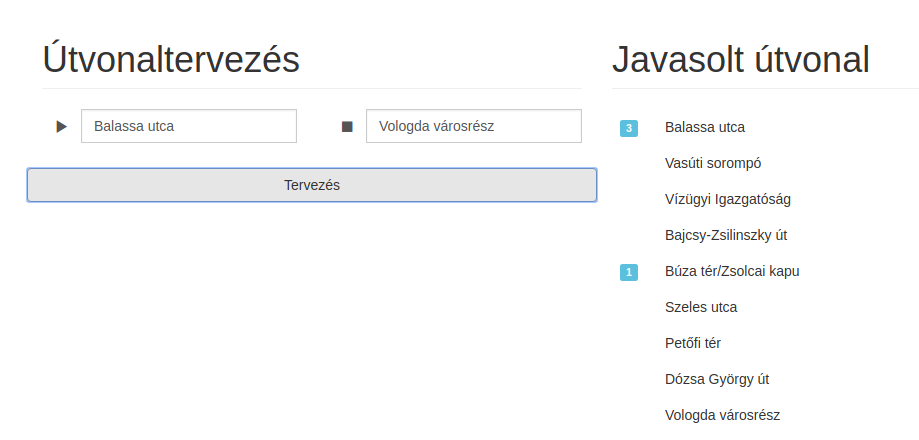
\includegraphics[scale=0.45]{kepek/trip_planner.png}
\caption{Útvonaltervezés}
\label{fig:trip_planner}
\end{figure}

\begin{figure}[h!]
\centering
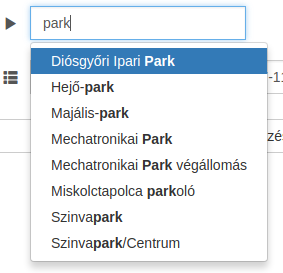
\includegraphics[scale=0.6]{kepek/autocomplete.png}
\caption{Automatikus kiegészítés a keresés segítéséhez}
\label{fig:autocomplete}
\end{figure}

\Section{Megvalósítás AngularJS segítségével}

A bemutatott felületek kialakítása AngularJS-sel történt. Az AngularJS kontrollerei kommunikálnak a szerverrel, az adatok nézeteken való megjelenítését biztosítják. Ezt az \texttt{app.js} fájl valósítja meg.
Az alkalmazás single-page application, ami azt jelenti, hogy egy oldal tartalma változik dinamikusan az alkalmazás használata során, nem teljesen különböző oldalak töltődnek le a szerverről. Különböző állapotok vannak definiálva, amiket a \texttt{\$stateProvider} modul kezel. Egy állapot definiálása a \texttt{\$stateProvider .state()} metódusával történik.
Egy állapot definiálása a következőképpen történik:
\begin{cpp}
.state("/trip", {
            url: "/trip/{trip_id:int}",
            templateUrl: "/static/partials/trip.html",
            controller: "tripController"
        })
\end{cpp}
Meg kell adni az állapot nevét, milyen URL-re aktiválódjon, melyik nézetet töltse be és melyik kontrollert használja hozzá.
Az \texttt{\$urlRouterProvider} segítségével létrehoztam egy úgynevezett \textit{otherwise} állapotot, ami akkor aktiválódik, ha az adott URL egyik állapot URL-ére sem illeszkedik. Ilyenkor egy erre figyelmeztető hibaüzenetet tartalmazó nézet töltődik be. Ezt mutatja \aref{fig:404}. ábra.

\begin{figure}[h!]
\centering
\frame{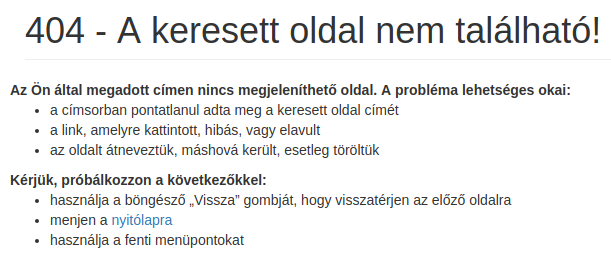
\includegraphics[scale=0.7]{kepek/404.png}}
\caption{404-es hibajelzés abban az esetben, ha a lap nem található}
\label{fig:404}
\end{figure}

A nézetek HTML-fájlokban vannak tárolva, ezek azonban nem teljes HTML-fájlok, csupán HTML-kódrészletek. Minden nézethez definiáltam egy kontrollert is, ezáltal jól elkülönítve az egyes állapotok kódjait.

Az elkészített nézetek és kontrollerek összefoglalása látható \aref{tab:routing}. táblázatban.

\begin{figure}[h!]
\centering
\begin{tabular}{|l|p{4cm}|l|}
\hline
\textbf{Nézet, \texttt{/static/partials/}} & \textbf{URL} & \textbf{Kontroller neve} \\
\hline
\texttt{home.html} & \texttt{/} & \texttt{-} \\
\hline
\texttt{list-routes.html} & \texttt{/list-routes} & \texttt{listRoutesController} \\
\hline
\texttt{trip.html} & \texttt{/trip/{trip\_id:int}} & \texttt{tripController} \\
\hline
\texttt{schedule.html} &
\texttt{/schedule/}

\texttt{:route\_short\_name/}

\texttt{\{direction\_id:int\}} & \texttt{scheduleController} \\
\hline
\texttt{trip-planner.html} & \texttt{/trip-planner} & \texttt{tripPlannerController} \\
\hline
\texttt{error-404.html} & \texttt{/error-404} & \texttt{-} \\
\hline
\end{tabular}
\caption{Routing: nézet, URL, kontroller}
\label{tab:routing}
\end{figure}

A \texttt{listRoutesController} a viszonylatokat kéri le a szervertől a viszonylatok típusa szerint csoportosítva. A megjelenített táblázatokban a különböző oszlopok szerinti rendezést és a bennük való keresést valósítja meg.
A \texttt{tripController} egy járat adatait kéri le a szervetől. Amennyiben hibás paramétert kap, a 404-es hibaoldalra irányít át.
A \texttt{scheduleController} az adatbázisban található dátumokat és egy viszonylat napi indulási adatait kéri le a szervertől. Alapértelmezetten az aktuális dátum szerinti menetrendet kérdezi le. Ha a nézeten a napválasztó legördülő menüből egy másik napot választ ki a felhasználó, akkor a kiválasztott nap menetrendjét kérdezi le.
A \texttt{tripPlannerController} lekérdezi az adatbázisban található megállók neveit, és a dátumokat. A hozzátartozó nézeten található formon bevitt adatokat validálja, ha hibásak, akkor megjeleníti a hibaüzenetet a nézeten. Ha a megadott adatok megfelelőek, elküldi azokat a szervernek, a válaszként kapott megtervezett útvonalat pedig megjeleníti a nézeten. Ha nem talált útvonalat az algoritmus, akkor szintén egy hibaüzenetet jelenít meg.

\Section{Térképadatok kezelése és megjelenítése}

A járatok útvonalának térképen történő megjelenítésére a Google Mapset használtam. Döntésemet az indokolta, hogy véleményem szerint a piacon jelenlévő térképszolgáltatások közül messze a Google-é a legfejlettebb, legtámogatottabb. A térkép programozására a Google Maps JavaScript API-t használtam. Ennek segítségével JavaScriptben írt kóddal tudjuk programozni a térképet. Számos funkciót kínál erre az API, én legfőképp az útvonalak kirajzolását és jelölőpontok megjelenítését használtam. Ahhoz, hogy oldalunkon használni tudjuk az API-t, be kell szereznünk egy úgynevezett API key-t. Ezt a következő oldalon tudjuk megtenni: \url{https://code.google.com/apis/console}.

Az oldalon létre kell hozni egy projektet, majd ki kell választani, hogy melyik API-ra van szükségünk. Én a Google Maps JavaScript API-t választottam ki, ezután meg is kaptam a szükséges kulcsot. Lehetőség van arra is, hogy lekorlátozzuk a kulcs használatát. Megadhatjuk, hogy mely domainnevekről használhatják a kulcsunkat. Ingyenesen napi 25 000 darab kérésünk lehet, ami egy átlagos forgalmú weboldal esetén elegendő. Ha azonban mégis átlépné az oldalunk ezt a napi limitet, akkor vásárolhatunk üzleti csomagot, amivel lehetőségünk van kibővíteni ezt a keretet. \Aref{fig:google_maps_api_1}. ábrán látható az adminisztrációs felületről egy kép.

\begin{figure}[h!]
\centering
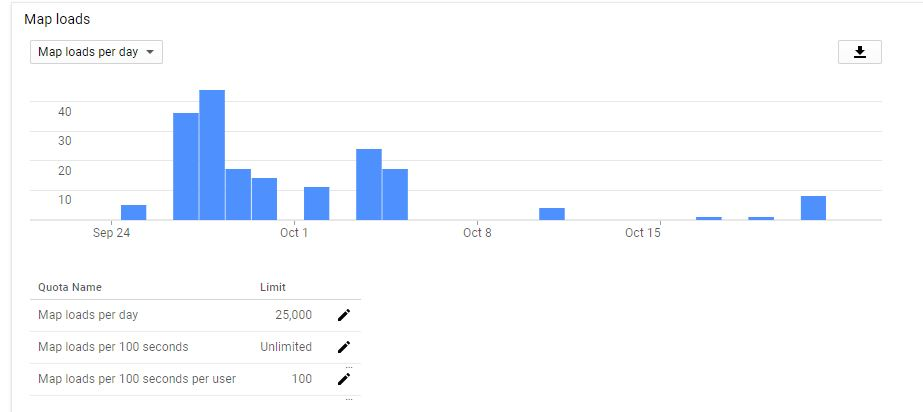
\includegraphics[scale=0.5]{kepek/google_maps_api_1.jpg}
\caption{Adminisztrációs felület}
\label{fig:google_maps_api_1}
\end{figure}

A fent hivatkozott honlapon a kérések monitorozására is lehetőségünk van. Ugyanezen a felületen beállíthatjuk a napi, a 100 másodpercenkénti és a 100 másodperc / felhasználó kérések limitjét (\ref{fig:google_maps_api_2}. ábra).

\begin{figure}[h!]
\centering
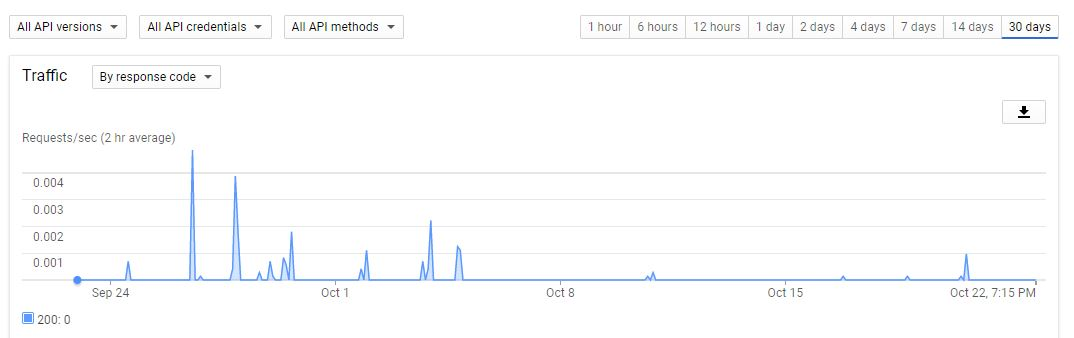
\includegraphics[scale=0.5]{kepek/google_maps_api_2.jpg}
\caption{Hálózati forgalom megjelenítése}
\label{fig:google_maps_api_2}
\end{figure}

Ha beszereztük a szükséges API key-t, akkor azt az oldalunkra be kell linkelni a következő módon:

\begin{verbatim}
<script src="https://maps.googleapis.com/maps/api/js?
key=IDE_KELL_A_KEY-T_BEMASOLNI&callback=drawMap"></script>
\end{verbatim}

A HTML-oldalon elhelyeztem egy \texttt{div}-et, ami a térképet tartalmazza, \texttt{id}-nak \texttt{map}-ot állítottam be. Létrehoztam egy scriptet, ami a \texttt{drawMap} függvényt tartalmazza, ez végzi a térkép manipulálását. A továbbiakban ennek a függvénynek néhány érdekesebb részét ismertetem.

A járatok útvonalai az adatbázisban tárolva vannak. Az adott járathoz tartozó GPS-koordinátákat lekérdezi a függvény a szervertől. Majd egy \texttt{for} cikluson belül ezekből úgynevezett \texttt{LatLng} objektumokat hoz létre a függvény, amit eltárol egy tömbben:

\begin{cpp}
var latlng = new google.maps.LatLng(
    value["shape_pt_lat"],
    value["shape_pt_lon"]
);
shapePoints.push(latlng);
\end{cpp}

Az első paraméter a szélességi, a második a hosszúsági koordináta. Még egy fontos dolog történik a \texttt{for} cikluson belül, egy \texttt{LatLngBounds} objektumot használok a térkép pozícionálásához.

\begin{cpp}
var bounds = new google.maps.LatLngBounds();
\end{cpp}

Ez \texttt{LatLng} objektumok által meghatározott téglalapot reprezentál. A \texttt{LatLngBounds} objektum \texttt{extend} metódusa hívódik meg a cikluson belül, paraméterként átadva az adott iterációban lévő \texttt{LatLng} objektumot, ezáltal a befoglaló téglalapban benne lesz az adott iteráció pontja is:

\begin{cpp}
bounds.extend(latlng);
\end{cpp}

A \texttt{for} ciklus lefutása után a \texttt{bounds} objektum az adott járat összes pontját tartalmazó minimális területű téglalapot fogja tartalmazni.
Hogy a pontokból útvonal legyen, ahhoz egy \texttt{Polyline} objektumot hoz létre a függvény, megadva a tömböt \texttt{path} property-ként. Egyéb beállítási lehetőségeink is vannak, én a vonal színét, átlátszóságát és vastagságát állítottam át, ezt mutatja a következő kódrészlet:

\begin{cpp}
var tripPath = new google.maps.Polyline({
                        path: shapePoints,
                        strokeColor: "#2cc124",
                        strokeOpacity: 0.8,
                        strokeWeight: 4
});
\end{cpp}

Miután ez az objektum is rendelkezésre áll, az útvonalat hozzárendeli a függvény a térképhez, valamint a térképet a befoglaló téglalapra pozícionálja:

\begin{cpp}
tripPath.setMap(map);
map.fitBounds(bounds);
\end{cpp}

A megállók megjelenítése \texttt{markerekkel} történik, megkülönböztetve a végállomásokat és a köztes megállókat. A végállomások tömött zöld körökkel, a köztes megállók zöld szegélyű, fehér kitöltésű körökkel vannak reprezentálva. Az útvonalhoz hasonlóan ebben az esetben is a szervertől lekérdezi a függvény a megállók koordinátáit. Ezt követően szintén egy \texttt{for} cikluson belül ezeken végigiterál, és iterációnként létrehoz egy-egy \texttt{LatLng} objektumot, illetve \texttt{markert}. A \texttt{marker} létrehozását láthatjuk a következő kódrészletben:

\begin{cpp}
var marker = new google.maps.Marker({
    position: latlng,
    icon: {
        path: google.maps.SymbolPath.CIRCLE,
        strokeColor: '#2cc124',
        fillColor: '#FFF',
        fillOpacity: 1,
        scale: 7
    },
    map: map,
    title: value["stop_name"]
});
\end{cpp}

Beállításra kerül a \texttt{marker} pozíciója a létrehozott \texttt{LatLng} objektumból. Az alapértelmezett ikon helyett az \texttt{icon} property megadásával használható más. Mint említettem, én köröket használok, megadva a szegély színét, a kitöltési színt, az átlátszóságot és az ikon nagyságát. A \texttt{markert} hozzá kell rendelni a térkép objektumhoz a \texttt{map} property megadásával. Végül én a \texttt{title} property-t is beállítom, a megálló nevét értékül adva neki. Ezáltal, ha rávisszük a kurzort az ikonra, akkor megjelenik a megálló neve. Ezenkívül \texttt{InfoWindow} ablakokat is használok, ezek akkor jönnek elő, ha egy \texttt{markerre} rákattintunk. Az adott megálló és a járat végállomásának a megállóját tartalmazza. Mindez jól látható \aref{fig:terkep}. ábrán.

\begin{figure}[h!]
\centering
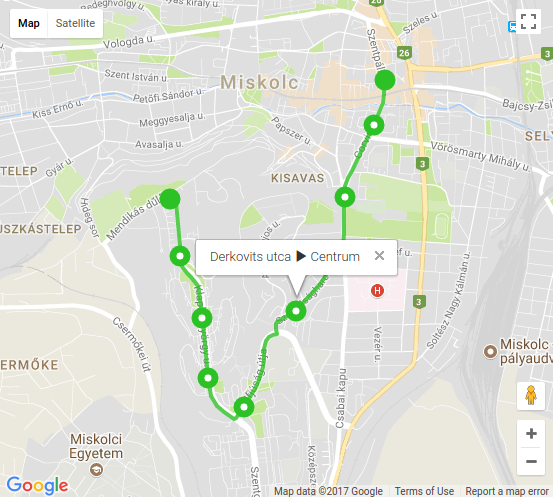
\includegraphics[scale=0.7]{kepek/terkep.png}
\caption{InfoWindow megjelenítése a Google-térképen}
\label{fig:terkep}
\end{figure}
